\documentclass[aps,prb,twocolumn,nofootinbib,superscriptaddress,floatfix]{revtex4-2}
\usepackage{amsmath,amssymb,amsthm,mathtools,bm}
\usepackage{booktabs}
\usepackage{graphicx}
\usepackage{tabularx}
\usepackage{array}
\usepackage[colorlinks=true,linkcolor=blue,citecolor=blue,urlcolor=blue]{hyperref}
\usepackage{microtype}

\hypersetup{
  pdftitle={Charge, covariance, and ensemble convergence in the class-A adaptive circuit},
  pdfauthor={Class-A fermionic adaptive-circuit project}
}

\graphicspath{
  {figures/}
  {../../../COLAB/colab_charge_fluctuations/analysis_outputs/total_charge_variance_cycle_derivative/N20_multi_geometry_nsh1_dwtrunc1_init-maxmix_S100_cycles-2Ny/figures/}
}

\newcommand{\Tr}{\operatorname{Tr}}
\newcommand{\tr}{\operatorname{tr}}
\newcommand{\Var}{\operatorname{Var}}
\newcommand{\Cov}{\operatorname{Cov}}
\newcommand{\dd}{\mathrm{d}}
\newcommand{\Nuc}{N_{\mathrm{uc}}}
\newcommand{\Vsp}{V}
\newcommand{\Qcov}{Q}
\newcommand{\Tconv}{T_{\mathrm{conv}}}
\newcommand{\Tint}{\tau_{\mathrm{int}}}

% Inline full-width material for the two-column grid.  This follows RevTeX's
% widetext machinery while replacing its decorative rules by invisible
% zero-width struts.  Unlike double-column floats, these blocks remain next to
% the discussion that introduces them.
\makeatletter
\newenvironment{wideblock}{%
  \par\ignorespaces
  \setbox\widetext@top\vbox{%
    \hb@xt@\hsize{\hfil\vrule\@width\z@\@height2\p@}%
  }%
  \setbox\widetext@bot\hb@xt@\hsize{%
    \vrule\@width\z@\@depth2\p@\hfil
  }%
  \onecolumngrid
  \vskip2\p@
  \dimen@\ht\widetext@top\advance\dimen@\dp\widetext@top
  \cleaders\box\widetext@top\vskip\dimen@
  \vskip1\p@
  \prep@math@patch
  \noindent\begin{minipage}{\textwidth}
}{%
  \end{minipage}
  \par
  \vskip1\p@
  \setbox\widetext@bot\vbox{%
    \hb@xt@\hsize{\hfil\box\widetext@bot}%
  }%
  \dimen@\ht\widetext@bot\advance\dimen@\dp\widetext@bot
  \cleaders\box\widetext@bot\vskip\dimen@
  \vskip2\p@
  \twocolumngrid\global\@ignoretrue
  \@endpetrue
}
\newenvironment{widefigure}{%
  \begin{wideblock}\def\@captype{figure}\centering
}{%
  \end{wideblock}
}
\newenvironment{widetable}{%
  \begin{wideblock}\def\@captype{table}\centering
}{%
  \end{wideblock}
}
\makeatother

\begin{document}

\title{Charge, covariance, and ensemble convergence in the class-A adaptive circuit}
\author{Internal campaign summary}
\affiliation{Class-A fermionic adaptive-circuit project}
\date{August 20, 2026}

\begin{abstract}
This note consolidates the charge-fluctuation and covariance-convergence
analysis of Born-rule class-A adaptive-circuit trajectories with a dynamical
domain wall.  The principal production ensembles have
$N_x=20$, $N_y=30,40,50$, two orbitals per unit cell, 100 trajectories,
$n_{\mathrm{shell}}=1$, hard domain-wall truncation, and $2N_y$ saved cycles.
We distinguish three logically different questions: purification of a
maximally mixed initial state, motion and stationarity of pure trajectories,
and statistical independence of cycle-resolved samples.  Global charge
variance and the root-mean-square normalized covariance norm reach an
operational transient threshold after only $15$--$16$ cycles, with no
detectable growth over the available $N_y$ range.  Spatial entropy contours,
however, reveal a fast active-bulk contraction with intrinsic time
$0.56$--$0.58$ cycles and an algebraic wall tail
$s_{\mathrm w}\sim t^{-\alpha_{\mathrm w}}$ with
$\alpha_{\mathrm w}=1.12$--$1.15$.  The wall reaches
$0.01$ bits per cell only after $46$--$57$ cycles.  Late-time
trajectory-to-trajectory occupancy variance is $97.2$--$97.3\%$ concentrated
on the exact wall rows, whereas the within-trajectory quantum variance is
not wall dominated.  Finally, block-stationarity and autocorrelation tests on
the default pure-state ensemble show that post-burn-in cycles are best viewed
as samples from a \emph{stationary, temporally correlated} ensemble.  The
charge-density autocorrelation time is only $1.3$--$1.4$ cycles, while the
long-range correlator exponent has $\tau_{\mathrm{int}}=14.8,20.3,24.1$
cycles, approximately $0.49N_y$.  Thus every retained cycle may contribute to
an ensemble estimate once stationarity is demonstrated, but neighboring cycles
must not be counted as independent samples.
\end{abstract}

\maketitle
\setcounter{tocdepth}{2}
\tableofcontents

\section{Scope and bottom line}
\label{sec:scope}

The original sequence of questions concerned charge variance, its cycle
derivative, Born-rule total-charge traces, Frobenius norms of covariance
matrices, spatial wall-versus-bulk resolution, and a defensible burn-in rule.
Those questions involve several different random variables and two different
initial-state ensembles.  The first purpose of this note is to prevent them
from being conflated.

There is a domain wall in every principal run analyzed here.  The $N_x=20$
production geometry has walls at $x=5$ and $x=15$, a topological active slab
$5\le x\le15$, and hard truncation of overcomplete Wannier (OW) modes across
the interfaces.  The run parameters are
$(\alpha_1,\alpha_2)=(1,30)$, $n_{\mathrm{shell}}=1$, ancillary filling
$\bar n_{\mathrm a}=1/2$, and the \texttt{perfect\_correction} protocol with
\texttt{postselect=False}.  A full cycle consists of OW-number measurements
with conditional fermionic-swap feedforward, followed by incoherent particle
redistribution and ancillary occupation measurement, as in
Ref.~\cite{Bhuiyan2026}.  Distinct OW stabilizers need not commute, and their
localized modes form an overcomplete rather than orthonormal Wannier basis.

The conclusions are observable dependent:
\begin{enumerate}
  \item The \emph{global purification transient} is short.  A sustained
  covariance-norm deficit below $10^{-3}$ together with a normalized norm rate
  below $10^{-4}$ per cycle occurs at cycles $15,15,16$ for
  $N_y=30,40,50$.
  \item The \emph{bulk purification transient} is shorter still.  The active
  bulk falls below $0.01$ bits per cell at cycle $4$ in all three
  spatial-entropy runs.
  \item The \emph{wall purification tail} is parametrically slower and is
  algebraic over cycles $5$--$30$.  Its $0.01$-bit threshold occurs at cycles
  $49,46,57$ for $16\times30$, $16\times32$, and $30\times40$.
  \item The rule ``burn in for $N_y$ cycles and measure on
  $[N_y,2N_y]$'' is a useful production convention, but it is not a theorem
  that every observable is stationary at cycle $N_y$.  The entanglement slope
  is stationary by a paired block test for all three $N_x=20$ sizes; the
  long-range correlator exponent still drifts for $N_y=30,40$ and is stationary
  for $N_y=50$.
  \item Stationarity is not independence.  Long-wavelength wall observables
  remain correlated for a substantial fraction of the measurement window.
  Uncertainty estimates must therefore resample whole trajectories or use
  autocorrelation-aware blocking rather than treating all trajectory--cycle
  pairs as independent.
\end{enumerate}

Accordingly, an endpoint measurement at cycle $2N_y$ is well inside the
observed low-entropy regime.  Pooling every cycle after burn-in is also
legitimate for a demonstrated stationary marginal distribution, but only as
correlated Monte Carlo sampling.  The maximally mixed purification campaign
is a special warning: its charge variance continues to decrease through
$[N_y,2N_y]$, so that particular time series is a transient diagnostic rather
than a stationary-ensemble sample.

\section{Geometry, trajectory ensembles, and provenance}
\label{sec:campaigns}

\subsection{Lattice and canonical correlation convention}

Let $\boldsymbol r=(x,y)$ label a unit cell and
$\mu\in\{1,2\}$ its two physical orbitals.  The physical fermions are
$\hat c_{\boldsymbol r,\mu}$, the number of unit cells is
$\Nuc=N_xN_y$, and the single-particle dimension is
\begin{equation}
 \Vsp=2\Nuc=2N_xN_y.
 \label{eq:volume}
\end{equation}
The total physical charge is
\begin{equation}
 \hat N_F=\sum_{\boldsymbol r,\mu}
 \hat c_{\boldsymbol r,\mu}^{\dagger}\hat c_{\boldsymbol r,\mu}.
\end{equation}
Following the project notation policy, a trajectory-resolved one-particle
correlation matrix is
\begin{equation}
 G_{ij}=\Tr\!\left(\hat\rho\,
 \hat c_i^\dagger\hat c_j\right),
 \qquad 0\le G\le\mathbf{1}_{\Vsp}.
 \label{eq:canonicalG}
\end{equation}
The archived simulation helpers call the shifted Hermitian covariance
``\texttt{G}.''  To avoid a collision, this note denotes that archived object by
\begin{equation}
 \Qcov=2G-\mathbf{1}_{\Vsp},
 \qquad G=\frac{\Qcov+\mathbf{1}_{\Vsp}}{2}.
 \label{eq:archivebridge}
\end{equation}
Thus every appearance of $G_tG_{t+1}-\mathbf{1}$ in the exploratory
discussion should be read as
$\Qcov_t\Qcov_{t+1}-\mathbf{1}_{\Vsp}$ in canonical notation.

\subsection{Born-rule trajectories and temporal samples}

For a measurement outcome $m$ with Kraus operator $\hat K_m$ and nonnegative
weight $w_m$, the simulation samples
\begin{equation}
 p_m=w_m\langle\!\langle\psi\rvert
 \hat K_m^\dagger\hat K_m
 \lvert\psi\rangle\!\rangle,
 \qquad
 \sum_m w_m\hat K_m^\dagger\hat K_m=\hat{\mathbf{1}}.
 \label{eq:born}
\end{equation}
A full record $\boldsymbol m=(m_1,m_2,\ldots)$ defines one member of the
many-body evolution-operator (mEO) ensemble
$\mathcal M_{\mathrm{mEO}}=\{\hat V_{\boldsymbol m}\}_{\boldsymbol m}$.
The 100 trajectory seeds are independent.  Successive cycles within a fixed
trajectory are not independent because they form a Markov chain on Gaussian
states.

For a trajectory observable $O_s(t)$, the cycle-resolved Born mean is
\begin{equation}
 \overline O(t)=\frac1S\sum_{s=1}^{S}O_s(t),\qquad S=100.
 \label{eq:bornmean}
\end{equation}
If the post-burn-in distribution is stationary, then the marginal
distribution of $O_s(t)$ is independent of $t$ and every retained cycle is a
valid, though correlated, draw from the same ensemble.  This distinction
between stationarity and independence is the central statistical point of
Sec.~\ref{sec:stationarity}.

\subsection{Campaign inventory}

\begin{widetable}
\caption{Data products used in this note.  All dynamics were previously run
through the canonical GPU entry point
\texttt{classA\_U1FGTN\_gpu.run\_markov\_circuit}; the present work is
analysis-only.  The entropy-contour sample counts are $10,10,25$ in the order
shown.}
\label{tab:campaigns}
\begin{tabularx}{\textwidth}{@{}>{\raggedright\arraybackslash}p{0.18\textwidth}>{\raggedright\arraybackslash}p{0.18\textwidth}X@{}}
\toprule
Ensemble & Geometry and sampling & Saved information and role \\
\midrule
Maximally mixed purification & $20\times(30,40,50)$; $S=100$;
$2N_y$ cycles & Total quantum charge variance, total entropy, local expected
charge, local quantum variance, and Chern marker.  Used for purification and
late-time charge localization. \\
Default pure-state streaming & $20\times(30,40,50)$; $S=100$;
$2N_y$ cycles & Entanglement and correlator fits, real-space Chern marker,
local expected charge, and successive covariance distance.  Used for
stationarity, autocorrelation, and trajectorywise motion. \\
Pure-state covariance snapshots & $16\times30$, $16\times40$; $S=10$;
cycles $5,10,20,50$ & Full sparse covariance snapshots.  Used for the
spatially reduced covariance pilot. \\
Maximally mixed entropy contours & $16\times30$ to cycle $50$,
$16\times32$ and $30\times40$ to cycle $100$ & Whole-system spatial entropy
contours.  Used for wall-versus-bulk purification fits and threshold times. \\
\bottomrule
\end{tabularx}
\end{widetable}

All principal $N_x=20$ runs use
$\texttt{dw\_loc}=(5,15)$, $\texttt{dw\_truncation=True}$,
$\texttt{sequence=raster\_y}$, complex128 arithmetic, and
$\texttt{postselect=False}$.  The $N_x=16$ snapshot constructor places the
walls at $x=4,12$.  Covariance histories were intentionally not retained in
the main campaigns; the requested global quantities were reconstructed from
streamed scalars, while spatial covariance diagnostics use the separate
sparse-snapshot pilot.

\subsection{Prior artifacts: this was not the first look}

The question whether rolling charge and Frobenius diagnostics had already
been plotted has an affirmative answer, but none of the older artifacts alone
contains the complete present comparison.  The May 6 notebook
\path{load_purification_charge_fluctuation_data_cpu_edited.ipynb}
used the same maximally mixed campaign and displayed rolling centered-charge
means and rolling percentage variances, with a different normalization.  The
older $20\times20$ notebook
\path{n20x20_dwtrunc_convergence_cpu.ipynb} plotted a successive
Frobenius-distance diagnostic for one size.  Finally,
\path{diagnose_perfect_correction_slope_excess_cpu.ipynb} used
\path{frob_successive_delta} alongside the entropy-slope excess.
The present bundle adds the three-size comparison, the exact normalization
identities, Born trace trajectories, spatial charge decomposition, explicit
wall/bulk purification fits, and the stationarity/autocorrelation test.

\section{Observables, normalization, and convergence estimators}
\label{sec:estimators}

\subsection{Within-trajectory quantum charge variance}

For a charge-conserving Gaussian state, Wick's theorem gives
\begin{equation}
 \Var_s(\hat N_F;t)
 =\tr\!\left[G_s(t)-G_s^2(t)\right].
 \label{eq:chargevariance}
\end{equation}
This is the quantum variance inside trajectory $s$.  It is not the variance of
the trajectory means.  The plotted cycle rate is
\begin{equation}
 \overline{\left|\partial_t\Var(\hat N_F)\right|}(t)
 =\frac1S\sum_s
 \left|\operatorname{gradient}_t\Var_s(\hat N_F;t)\right|,
 \label{eq:chargevariancerate}
\end{equation}
where the archived analysis uses \texttt{numpy.gradient} on the integer cycle
grid with second-order edge handling.  Both quantities are shown on logarithmic
$y$ axes.

\subsection{Expected total charge and trajectory-to-trajectory variance}

The expected total charge on trajectory $s$ is
\begin{equation}
 n_s(t)=\tr G_s(t)=\langle\hat N_F\rangle_s.
 \label{eq:trace}
\end{equation}
Half filling is $\Vsp/2=N_xN_y$, whereas the largest possible charge is
$\Vsp=2N_xN_y$.  The requested normalized displacement is therefore
\begin{equation}
 q_s(t)=\frac{n_s(t)-\Vsp/2}{\Vsp}.
 \label{eq:qnormalized}
\end{equation}
The Born mean $\overline q(t)$ measures the ensemble's fractional offset from
half filling.  Two distinct measures of its spread are useful:
\begin{align}
 v_N(t)&=\frac{\Var_s[n_s(t)]}{\Vsp},
 \label{eq:extensivevariance}\\
 \sigma_{n/\Vsp}(t)&=\frac{\sqrt{\Var_s[n_s(t)]}}{\Vsp}.
 \label{eq:densitysd}
\end{align}
The first is an extensive-variance density and is what the trace-variance panel
plots.  The second is the standard deviation of the fractional filling and is
the more direct ``typical occupancy deviation.''  Dividing the variance only
by $\Vsp$ should not be confused with the variance of $n_s/\Vsp$, which would
contain $\Vsp^2$ in the denominator.

\subsection{Covariance Frobenius norm and the correct size collapse}

Equations~\eqref{eq:archivebridge} and \eqref{eq:chargevariance} imply the exact
trajectorywise identity
\begin{equation}
 \Var_s(\hat N_F;t)=
 \frac{\Vsp-\tr\Qcov_s^2(t)}4
 =\frac{\Vsp-\lVert\Qcov_s(t)\rVert_F^2}{4},
 \label{eq:normidentity}
\end{equation}
because $\Qcov$ is Hermitian.  Hence
\begin{equation}
 \lVert\Qcov_s(t)\rVert_F=
 \sqrt{\Vsp-4\Var_s(\hat N_F;t)}.
 \label{eq:normreconstruction}
\end{equation}
For a pure number-conserving Gaussian state,
$\Qcov^2=\mathbf{1}_{\Vsp}$ and
$\lVert\Qcov\rVert_F=\sqrt{\Vsp}$.  This resolves the normalization puzzle:
\begin{align}
 \frac{\lVert\Qcov\rVert_F}{\Vsp}
 &\longrightarrow \Vsp^{-1/2},
 \label{eq:wrongnorm}\\
 \frac{\lVert\Qcov\rVert_F}{\sqrt{\Vsp}}
 &\longrightarrow 1.
 \label{eq:rmsnorm}
\end{align}
Dividing a Frobenius norm by $2N_xN_y=\Vsp$ therefore necessarily makes its
saturated value smaller at larger $N_y$: a Frobenius norm is root-extensive,
not extensive.  Equation~\eqref{eq:rmsnorm} is the root-mean-square (RMS)
spectral normalization that removes this trivial scaling.

Define the normalized deficit and absolute norm rate by
\begin{align}
 d_F(t)&=1-
 \frac{\overline{\lVert\Qcov(t)\rVert_F}}{\sqrt{\Vsp}},
 \label{eq:frobdeficit}\\
 r_F(t)&=\frac{1}{\sqrt{\Vsp}}
 \overline{\left|\partial_t\lVert\Qcov(t)\rVert_F\right|}.
 \label{eq:frobrate}
\end{align}
The displayed $r_F$ uses a centered rolling mean with width five; all threshold
tests retain the documented raw trajectory aggregation before applying that
same deterministic rolling operation.

\subsection{Adjacent-cycle covariance motion}

For the pure-state streaming ensemble, $\Qcov_t$ is a Hermitian involution.
Consequently,
\begin{align}
 \Qcov_{t-1}\Qcov_t-\mathbf{1}_{\Vsp}
 &=\Qcov_{t-1}(\Qcov_t-\Qcov_{t-1}),\nonumber\\
 \left\lVert\Qcov_{t-1}\Qcov_t-\mathbf{1}_{\Vsp}\right\rVert_F
 &=\left\lVert\Qcov_t-\Qcov_{t-1}\right\rVert_F.
 \label{eq:productidentity}
\end{align}
Left multiplication by $\Qcov_{t-1}$ preserves the Frobenius norm.  The
streamed scalar \texttt{frob\_successive\_delta} is therefore exactly the
requested adjacent-product residual, without saving $\Qcov_t$ itself.  A
nonzero plateau of this quantity means that trajectories continue moving; it
does not mean the ensemble distribution is nonstationary.

\subsection{Spatial reduction and the origin of \texorpdfstring{$R_x$}{Rx}}

Let $P_x$ retain both orbitals at a fixed $x$ row for every $y$.  The principal
submatrix
\begin{equation}
 \Qcov_x(t)=P_x\Qcov(t)P_x
 \label{eq:reducedQ}
\end{equation}
is the shifted covariance matrix of the Gaussian reduced state obtained by
tracing out all other $x$ rows.  It acts on $2N_y$ modes.  The spatially
resolved temporal rate introduced in the exploratory analysis is
\begin{equation}
 R_x(t_a,t_b)=
 \frac{\left\lVert\Qcov_x(t_b)-\Qcov_x(t_a)\right\rVert_F}
 {(t_b-t_a)\sqrt{2N_y}}.
 \label{eq:Rx}
\end{equation}
Thus $R_x$ is not a new physical operator.  It is simply the finite-difference
speed of the reduced covariance on row $x$, with the same RMS spectral
normalization used globally.  The partial trace generally makes the reduced
state mixed even when the full trajectory is pure.  Its mixedness diagnostic is
\begin{equation}
 M_x(t)=\frac{\left\lVert\Qcov_x^2(t)-\mathbf{1}_{2N_y}\right\rVert_F}
 {\sqrt{2N_y}}.
 \label{eq:Mx}
\end{equation}
Because $M_x$ need not vanish in a stationary reduced state, the local product
residual
$\lVert\Qcov_x(t_a)\Qcov_x(t_b)-\mathbf{1}_{2N_y}\rVert_F$ would mix temporal
motion with ordinary reduced-state mixedness and is not used as a convergence
criterion.

\subsection{Regional entropy and convergence thresholds}

Let $s(\boldsymbol r,t)$ be the trajectory-averaged entanglement contour in
bits.  The wall entropy density averages $s$ over the two exact wall rows and
all $y$; the active-bulk density averages rows inside the topological slab at
least two rows away from either wall.  The hard-truncated exterior is excluded.
The wall is compared on cycles $5$--$30$ to
\begin{align}
 s_{\mathrm w}(t)&=A_{\mathrm w}t^{-\alpha_{\mathrm w}},
 \label{eq:wallpower}\\
 s_{\mathrm w}(t)&=A_{\mathrm w}e^{-t/\tau_{\mathrm w}},
 \label{eq:wallexponential}
\end{align}
using ordinary least squares in log space.  The bulk is described by
\begin{equation}
 s_{\mathrm b}(t)=A_{\mathrm b}e^{-t/\tau_{\mathrm b}}
 +B_{\mathrm b}t^{-\alpha_{\mathrm w}},
 \label{eq:bulkmodel}
\end{equation}
where $\alpha_{\mathrm w}$ is fixed to the wall fit.  A threshold time
$T_R(\epsilon)$ is the first saved cycle after which the regional entropy
density remains below $\epsilon$ for every later saved cycle.

\subsection{Stationarity and autocorrelation estimators}

For each observable $O_s(t)$, the measurement window is the inclusive set
$N_y\le t\le2N_y$.  It is divided at $3N_y/2$.  The paired block difference
for trajectory $s$ is
\begin{equation}
 d_s=\langle O_s\rangle_{[3N_y/2,2N_y]}
 -\langle O_s\rangle_{[N_y,3N_y/2)}.
 \label{eq:blockdifference}
\end{equation}
The reported 95\% interval for $\overline d$ is a percentile interval from
2000 resamplings of complete trajectories.  This is a direct test for drift
between the early and late halves of the proposed measurement window.

To estimate temporal dependence without confusing it with common drift, define
residuals
\begin{equation}
 \delta O_s(t)=O_s(t)-\overline O(t).
\end{equation}
Their pooled lag correlation is
\begin{equation}
 \rho_O(k)=
 \frac{\sum_{s,t}\delta O_s(t)\delta O_s(t+k)}
 {\sqrt{\sum_{s,t}\delta O_s^2(t)
 \sum_{s,t}\delta O_s^2(t+k)}}.
 \label{eq:acf}
\end{equation}
The integrated autocorrelation time uses the initial-positive sequence,
\begin{equation}
 \Tint[O]=1+2\sum_{k=1}^{k_+}\rho_O(k),
 \label{eq:tauint}
\end{equation}
where $k_+$ ends immediately before the first nonpositive lag.  The approximate
number of independent-equivalent samples is
\begin{equation}
 N_{\mathrm{eff}}[O]\simeq
 \frac{S(N_y+1)}{\Tint[O]}.
 \label{eq:neff}
\end{equation}
This is a diagnostic, not a proof that every functional of the full covariance
has equilibrated.

\begin{widetable}
\caption{Normalization dictionary.  The archive calls the shifted covariance
$\Qcov$ by the name \texttt{G}; Eq.~\eqref{eq:archivebridge} is the exact
translation to canonical paper notation.}
\label{tab:normalizations}
\begin{tabularx}{\textwidth}{@{}>{\raggedright\arraybackslash}p{0.23\textwidth}>{\raggedright\arraybackslash}p{0.28\textwidth}X@{}}
\toprule
Quantity & Definition & Interpretation \\
\midrule
Charge-density offset & $(\tr G-\Vsp/2)/\Vsp$ & Fraction of the total charge
capacity by which a trajectory or Born mean differs from half filling. \\
Trajectory charge variance density & $\Var_s(\tr G)/\Vsp$ & Extensive
between-trajectory variance per single-particle mode. \\
Fractional-filling standard deviation & $\sqrt{\Var_s(\tr G)}/\Vsp$ & Typical
trajectory-to-trajectory deviation of the filling fraction. \\
Quantum charge variance density & $\tr(G-G^2)/\Vsp$ & Within-trajectory
number uncertainty per mode. \\
RMS covariance norm & $\lVert\Qcov\rVert_F/\sqrt{\Vsp}$ & Intensive purity
diagnostic with pure-state ceiling one. \\
Adjacent covariance step & $\lVert\Qcov_t-\Qcov_{t-1}\rVert_F/\sqrt{\Vsp}$ &
Trajectorywise motion per cycle; not a stationarity test by itself. \\
\bottomrule
\end{tabularx}
\end{widetable}

\section{Global charge sharpening and covariance purification}
\label{sec:global}

\subsection{Charge variance and its absolute cycle derivative}

\begin{widefigure}
\centering
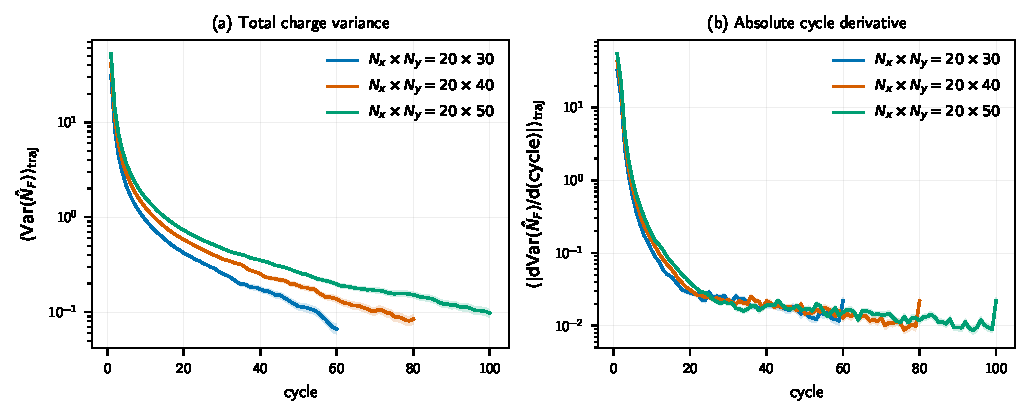
\includegraphics[width=0.98\textwidth]{total_charge_variance_and_cycle_derivative.pdf}
\caption{Maximally mixed purification ensemble with 100 Born-rule trajectories.
Left: sample-averaged within-trajectory quantum variance
$\overline{\Var(\hat N_F)}$.  Right: trajectory mean of the absolute cycle
derivative in Eq.~\eqref{eq:chargevariancerate}.  Both $y$ axes are logarithmic;
the narrow bands are one standard error.  No smoothing is applied.  The domain
wall and hard truncation are present in all three sizes.}
\label{fig:chargevariance}
\end{widefigure}

Figure~\ref{fig:chargevariance} shows a fast initial collapse followed by a
much slower tail.  At the final saved cycle, the unnormalized means are
$0.06647$, $0.08464$, and $0.09733$ for $N_y=30,40,50$.  The corresponding
densities are $5.54\times10^{-5}$, $5.29\times10^{-5}$, and
$4.87\times10^{-5}$ per single-particle mode.  The curves therefore grow
weakly with $N_y$ only because the observable is extensive; the final density
slightly decreases over this range.

The absolute derivative falls from $O(10^1)$ in the first cycle to an
$O(10^{-2})$ noisy late-time floor.  Taking the absolute value before averaging
is essential: a derivative of the ensemble mean could hide trajectorywise
motion by cancellation.  The remaining floor also explains why convergence
must be defined with a documented tolerance rather than the impossible
condition of a numerically zero derivative.

\subsection{Frobenius norm and operational global transient}

\begin{widefigure}
\centering
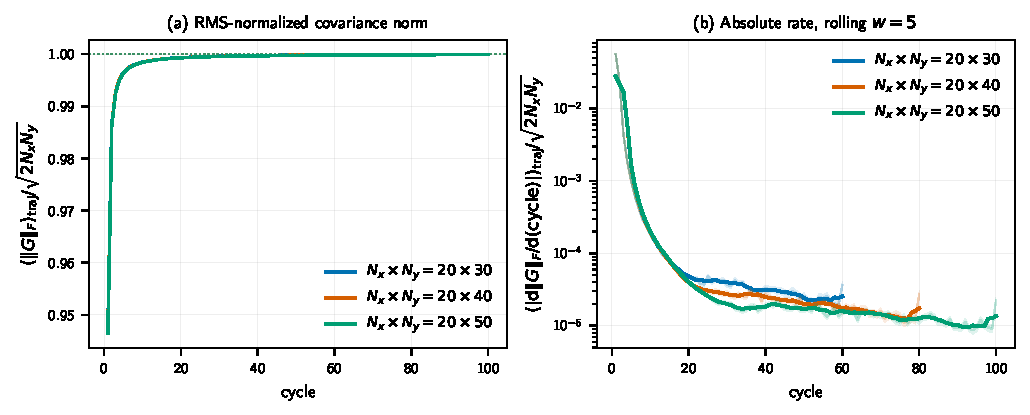
\includegraphics[width=0.98\textwidth]{frobenius_norm_and_cycle_derivative.pdf}
\caption{The same maximally mixed ensemble expressed through the exact norm
identity \eqref{eq:normreconstruction}.  Left: RMS-normalized covariance norm,
whose pure-state ceiling is one.  Right: its RMS-normalized absolute rate on a
logarithmic axis.  Faint curves and bands are unsmoothed means and standard
errors; thick curves are centered rolling means with $W=5$.}
\label{fig:frobenius}
\end{widefigure}

The apparent size dependence that resulted from dividing
$\lVert\Qcov\rVert_F$ by $2N_xN_y$ is absent in
Fig.~\ref{fig:frobenius}, because the correct denominator is
$\sqrt{2N_xN_y}$.  All three curves approach the common pure-state ceiling.
The late 20\%-of-run mean deficits are
$1.61\times10^{-4}$, $1.23\times10^{-4}$, and $1.21\times10^{-4}$.

The operational global time is
\begin{equation}
 \Tconv^{(F)}=max\left\{
 T[d_F\le10^{-3}],\;T[r_F^{(W=5)}\le10^{-4}/\text{cycle}]
 \right\},
 \label{eq:globalTconv}
\end{equation}
where each inequality must remain satisfied at every later saved cycle.
Trajectory bootstrapping with 2000 repetitions gives Table~\ref{tab:global}.

\begin{widetable}
\caption{Global covariance-purification convergence.  Confidence intervals
are percentile intervals from resampling complete trajectories.}
\label{tab:global}
\begin{ruledtabular}
\begin{tabular}{c c c c c c}
$N_y$ & $T[d_F\le10^{-3}]$ & $T[r_F\le10^{-4}]$ & $\Tconv^{(F)}$
& late $\overline d_F$ & final $\overline{\Var(\hat N_F)}$ \\
\hline
30 & $15\,[15,15]$ & $14\,[14,14]$ & $15\,[15,15]$ &
$1.61\times10^{-4}$ & $0.06647$ \\
40 & $15\,[15,16]$ & $14\,[14,14]$ & $15\,[15,16]$ &
$1.23\times10^{-4}$ & $0.08464$ \\
50 & $16\,[15,16]$ & $14\,[14,14]$ & $16\,[15,16]$ &
$1.21\times10^{-4}$ & $0.09733$ \\
\end{tabular}
\end{ruledtabular}
\end{widetable}

Within $30\le N_y\le50$ and fixed $N_x=20$, the global scalar transient is
indistinguishable from an $O(1)$ cycle count with respect to $N_y$.  This is a
finite-range statement, not an asymptotic proof.  More importantly, it says
nothing by itself about a spatially localized slow mode: a boundary occupies a
vanishing fraction of the full two-dimensional volume and can be hidden in a
global Frobenius average.

\section{Born-rule total charge: mean, spread, and stationarity}
\label{sec:borncharge}

\begin{widefigure}
\centering
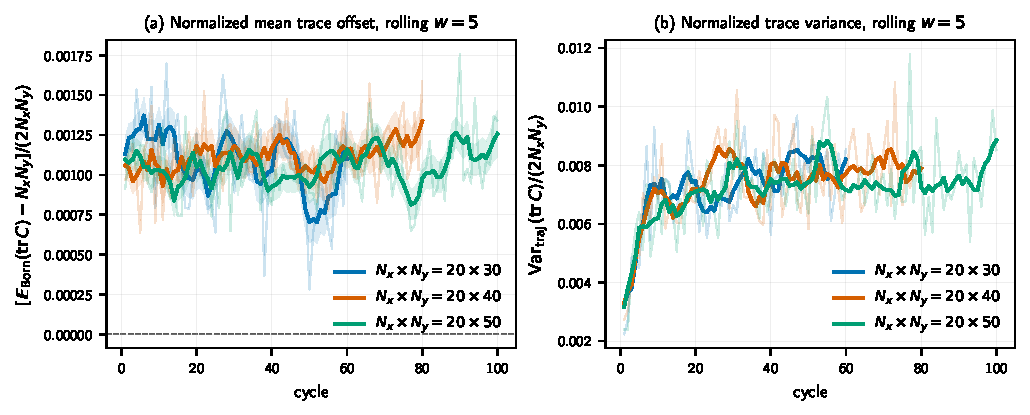
\includegraphics[width=0.98\textwidth]{born_rule_total_charge_trace_mean_and_variance.pdf}
\caption{Born-rule total-charge trace in the maximally mixed purification
ensemble.  Left: $[\overline{\tr G}-\Vsp/2]/\Vsp$.  Right:
$\Var_s(\tr G)/\Vsp$.  Thick lines are centered rolling means with $W=5$;
faint lines and bands show unsmoothed values and their standard errors.  The
nonzero right panel demonstrates that \texttt{perfect\_correction} does not
place all trajectories in one fixed-charge sector.}
\label{fig:borntrace}
\end{widefigure}

The ensemble mean remains close to half filling but not exactly at it.  In the
late half $N_y<t\le2N_y$, the mean fractional offsets are approximately
$1.01$, $1.14$, and $1.09$ parts in $10^3$.  The trajectory variance density
is nearly size independent, about $7.6$--$7.9\times10^{-3}$.  The typical
fractional-filling deviation in Eq.~\eqref{eq:densitysd}, however, decreases as
$\Vsp^{-1/2}$ from $2.56\times10^{-3}$ to $1.95\times10^{-3}$.

\begin{widetable}
\caption{Late-window total-charge and quantum-variance statistics for the
maximally mixed ensemble, averaged over cycles $N_y+1$ through $2N_y$.
$\sigma_{n/\Vsp}$ is the typical deviation of the fractional occupancy across
trajectories.}
\label{tab:chargewindow}
\begin{ruledtabular}
\begin{tabular}{c c c c c c}
$N_y$ & $\overline q$ & $\Var_s(n)/\Vsp$ & $\sigma_{n/\Vsp}$ &
$\overline{\Var(\hat N_F)}$ & $\overline{\Var(\hat N_F)}/\Vsp$ \\
\hline
30 & $1.007\times10^{-3}$ & $7.872\times10^{-3}$ & $2.561\times10^{-3}$
& $0.1464$ & $1.220\times10^{-4}$ \\
40 & $1.139\times10^{-3}$ & $7.830\times10^{-3}$ & $2.212\times10^{-3}$
& $0.1455$ & $9.092\times10^{-5}$ \\
50 & $1.087\times10^{-3}$ & $7.634\times10^{-3}$ & $1.954\times10^{-3}$
& $0.1607$ & $8.034\times10^{-5}$ \\
\end{tabular}
\end{ruledtabular}
\end{widetable}

The expected occupancy is therefore tightly bounded empirically around half
filling: the mean bias is about $0.1\%$ of capacity and a typical trajectory is
within roughly $0.2$--$0.26\%$ of capacity.  These are finite-sample statistics,
not rigorous probability bounds.  They can support a statement about the
observed ensemble but cannot prove confinement for all times or sizes.

The slowly falling quantum variance in Fig.~\ref{fig:chargevariance} supplies a
second caution.  In the maxmix ensemble, its first-to-second half changes over
$[N_y,2N_y]$ are
$-7.31\times10^{-5}$, $-5.49\times10^{-5}$, and
$-3.47\times10^{-5}$ after division by $\Vsp$, with bootstrap intervals that
exclude zero.  Thus the expected total charge is approximately stationary by
$N_y$, but the state is still purifying weakly.  The entire window must not be
called a stationary charge-variance ensemble without this qualification.

\section{Where the charge fluctuations live}
\label{sec:spatialcharge}

\subsection{Three inequivalent spatial profiles}

Define the cell occupation
\begin{equation}
 n_s(x,y,t)=\sum_{\mu=1}^{2}
 [G_s(t)]_{(x,y,\mu),(x,y,\mu)}.
\end{equation}
At half filling its reference value is one.  The late-time spatial analysis
uses cycles $N_y+1$ through $2N_y$, averages along $y$, and keeps separate:
\begin{align}
 b(x)&=\left|\overline{n(x,y,t)}-1\right|,\nonumber\\
 v_{\mathrm{traj}}(x)&=\overline{
 [n_s(x,y,t)-\overline n(x,y,t)]^2},\nonumber\\
 v_{\mathrm q}(x)&=\overline{\Var_s[\hat N_{x,y}]}.
 \label{eq:spatialprofiles}
\end{align}
The first is ensemble bias, the second is between-trajectory fluctuation of an
expectation value, and the third is quantum fluctuation inside each trajectory.

\begin{widefigure}
\centering
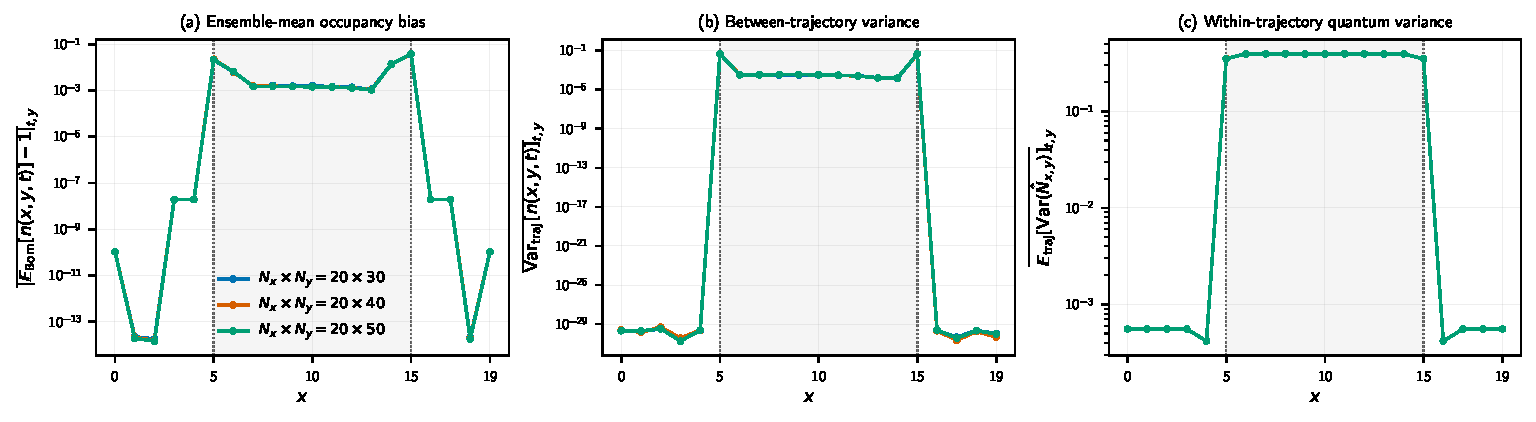
\includegraphics[width=0.99\textwidth]{late_time_boundary_bulk_charge_profiles.pdf}
\caption{Late-window charge profiles in the $N_x=20$ maxmix ensemble.  Panel
(a) shows the absolute bias of the Born mean from one particle per cell; panel
(b) shows between-trajectory variance of the expected cell occupancy; panel
(c) shows the within-trajectory quantum variance.  The shaded active slab is
$5\le x\le15$, and the dotted lines are its two domain walls.  Curves for all
three $N_y$ values nearly collapse.}
\label{fig:chargeprofiles}
\end{widefigure}

Figure~\ref{fig:chargeprofiles} supports a strong but carefully delimited wall
statement.  The ensemble-mean bias and especially the trajectory-to-trajectory
variance are wall localized.  The within-trajectory quantum variance is not:
it is broad and nearly uniform across the active slab.

\begin{widetable}
\caption{Late-window wall localization.  ``Exact wall'' uses $x=5,15$;
``distance $\le1$'' adds their neighboring rows.  The wall/bulk density ratio
uses wall-adjacent rows $x=5,6,14,15$ and active-bulk rows $x=7,\ldots,13$.}
\label{tab:localization}
\begin{ruledtabular}
\begin{tabular}{c l c c c}
$N_y$ & Metric & exact-wall capture & distance-$\le1$ capture & wall/bulk ratio \\
\hline
30 & mean occupancy bias & $0.657$ & $0.884$ & $13.36$ \\
40 & mean occupancy bias & $0.668$ & $0.891$ & $14.30$ \\
50 & mean occupancy bias & $0.665$ & $0.892$ & $14.40$ \\
30 & trajectory occupancy variance & $0.973$ & $0.978$ & $77.91$ \\
40 & trajectory occupancy variance & $0.972$ & $0.978$ & $76.88$ \\
50 & trajectory occupancy variance & $0.973$ & $0.978$ & $78.00$ \\
30 & within-trajectory quantum variance & $0.165$ & $0.351$ & $0.946$ \\
40 & within-trajectory quantum variance & $0.165$ & $0.350$ & $0.945$ \\
50 & within-trajectory quantum variance & $0.165$ & $0.350$ & $0.945$ \\
\end{tabular}
\end{ruledtabular}
\end{widetable}

More than $99.9999\%$ of the first two profiles lies inside the active slab.
That near-zero exterior is partly imposed by hard domain-wall truncation and
must not be presented as an emergent proof of localization.  The robust
interior statement is instead that approximately $97.3\%$ of the
between-trajectory occupancy variance lies on the two exact wall rows and that
the wall-row variance density is about $77$--$78$ times the active-bulk value.
The phrase ``most charge fluctuations come from the boundary'' is therefore
correct for ensemble-to-ensemble occupancy fluctuations, but false for the
within-trajectory quantum charge variance.

\subsection{Reduced-covariance pilot}

\begin{widefigure}
\centering
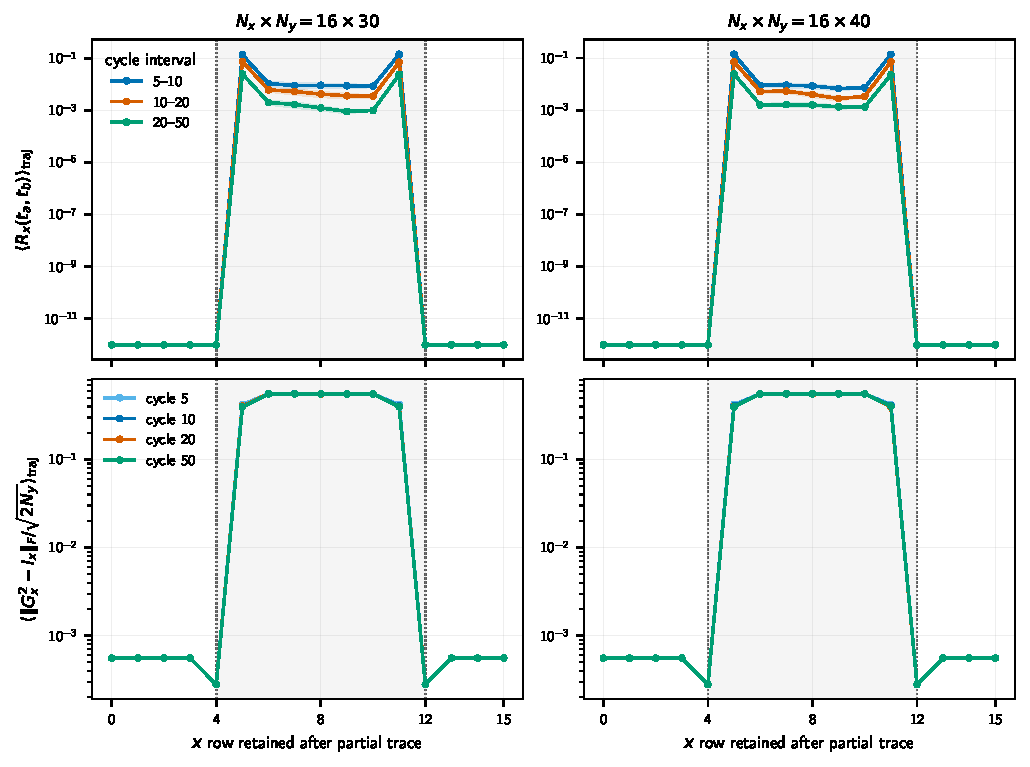
\includegraphics[width=0.86\textwidth]{spatial_reduced_covariance_convergence_pilot.pdf}
\caption{Sparse-snapshot pure-state pilot for $N_x=16$.  Top row: the reduced
covariance rate $R_x(t_a,t_b)$ of Eq.~\eqref{eq:Rx}; bottom row: reduced-state
mixedness $M_x(t)$ of Eq.~\eqref{eq:Mx}.  Dotted lines mark the walls at
$x=4,12$.  The rate is $7.5$--$8.9$ times larger on active wall rows than in
the active bulk over the three observed intervals.  Ten trajectories and only
four snapshot cycles make this descriptive rather than a precision scaling
study.}
\label{fig:reducedcovariance}
\end{widefigure}

The top panels of Fig.~\ref{fig:reducedcovariance} give the desired spatial
resolution of covariance motion after tracing out all other $x$ rows.  In the
$20$--$50$ interval the wall-to-bulk rate ratios are $8.94$ for
$16\times30$ and $7.92$ for $16\times40$.  The active-bulk rate has already
fallen to $1.36\times10^{-3}$ and $1.49\times10^{-3}$ per cycle, whereas the
wall remains at $1.22\times10^{-2}$ and $1.18\times10^{-2}$.

The bottom panels explain why reduced-state mixedness cannot replace a temporal
rate.  $M_x$ remains $O(1)$ inside the active slab even while successive curves
nearly coincide, because tracing out the other rows creates a mixed subsystem.
Mixedness is a property of the reduced state; $R_x$ is the finite-difference
convergence diagnostic.

\section{Fast bulk and algebraic wall purification}
\label{sec:wallbulk}

\subsection{Sparse covariance-rate evidence}

\begin{widefigure}
\centering
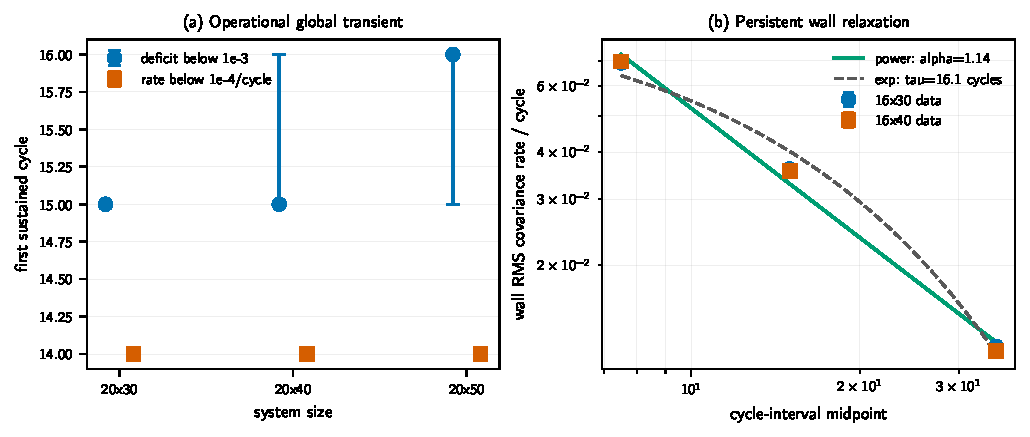
\includegraphics[width=0.98\textwidth]{quantitative_transient_timescale_and_wall_decay.pdf}
\caption{Two complementary convergence summaries.  Left: the global
Frobenius thresholds defining Eq.~\eqref{eq:globalTconv}.  Right: common-amplitude
fits of the six sparse wall-rate points from the reduced-covariance pilot to a
power law and an exponential.  The wall-rate power fit gives
$\alpha=1.144$; the exponential gives $\tau=16.1$ cycles.}
\label{fig:quantitative}
\end{widefigure}

The sparse $R_x$ pilot favors a power law over an exponential by
$\Delta\mathrm{AICc}=3.52$; in 2000 paired trajectory bootstraps, the power law
has lower AICc in $97.45\%$ of resamples.  The bootstrap interval for the model
difference narrowly includes zero, so this is supporting rather than decisive
evidence.  The full entropy-contour histories provide the stronger test.

\subsection{Cycle-resolved entropy contours}

\begin{widefigure}
\centering
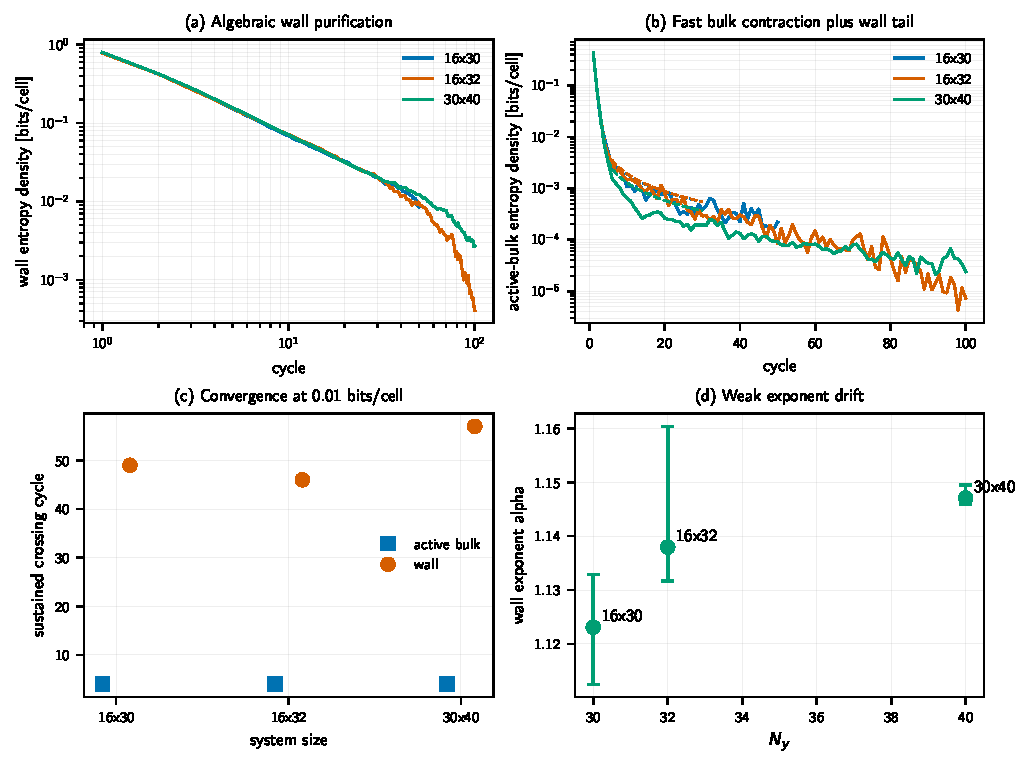
\includegraphics[width=0.86\textwidth]{wall_bulk_purification_convergence_and_scaling.pdf}
\caption{Spatially resolved purification from maximally mixed initial states.
(a) Wall entropy density on log--log axes.  (b) Active-bulk entropy density on
a logarithmic $y$ axis.  (c) first sustained crossing of $0.01$ bits per cell.
(d) wall power-law exponent from cycles $5$--$30$; error bars show the range
obtained by moving the fit onset among cycles $3,5,8,10$, not a statistical
confidence interval.  The $16\times30$ run ends at cycle $50$; the other two
end at cycle $100$.}
\label{fig:wallbulk}
\end{widefigure}

The wall curves in Fig.~\ref{fig:wallbulk}(a) are nearly straight over more
than a decade on log--log axes.  Direct wall fits give
$\alpha_{\mathrm w}=1.1231,1.1380,1.1471$, with log-space
$R^2=0.99929,0.99847,0.99989$ for the three geometries.  Replacing the power
law by an exponential raises AICc by $112.9$, $91.1$, and $138.8$,
respectively.  In contrast, the intrinsic bulk component in
Eq.~\eqref{eq:bulkmodel} has
$\tau_{\mathrm b}=0.564,0.570,0.585$ cycles.  The subsequent weak bulk tail is
well described as leakage of the same wall power law into the regional
average.

\begin{widetable}
\caption{Wall/bulk purification statistics.  The $2N_y$ entropy density is
reported at cycle $50$ for $16\times30$ because that run was not saved to
cycle $60$.  A dash denotes a right-censored threshold.}
\label{tab:wallbulk}
\begin{ruledtabular}
\begin{tabular}{c c c c c c c}
Geometry & $\alpha_{\mathrm w}$ & $\Delta\mathrm{AICc}_{\exp-\mathrm{pow}}$
& $\tau_{\mathrm b}$ & $T_{\mathrm w}(10^{-2})$
& $T_{\mathrm b}(10^{-2})$ & $s_{\mathrm w}$ near $2N_y$ \\
\hline
$16\times30$ & $1.123$ & $112.9$ & $0.564$ & $49$ & $4$ &
$8.52\times10^{-3}$ at $t=50$ \\
$16\times32$ & $1.138$ & $91.1$ & $0.570$ & $46$ & $4$ &
$4.57\times10^{-3}$ at $t=64$ \\
$30\times40$ & $1.147$ & $138.8$ & $0.585$ & $57$ & $4$ &
$4.85\times10^{-3}$ at $t=80$ \\
\end{tabular}
\end{ruledtabular}
\end{widetable}

These data explain why there is no unique ``the transient time.''  A global
norm gives $15$--$16$ cycles; active-bulk entropy gives four cycles at the
$0.01$-bit tolerance; the wall requires about $50$--$60$ cycles.  Because the
wall decay is algebraic, its tolerance-dependent time behaves approximately as
\begin{equation}
 T_{\mathrm w}(\epsilon)\sim
 \left(\frac{A_{\mathrm w}}{\epsilon}\right)^{1/\alpha_{\mathrm w}},
 \label{eq:tolerancewalltime}
\end{equation}
rather than being characterized by one exponential time constant.

The existing geometries do not determine an asymptotic system-size exponent for
$T_{\mathrm w}$.  Only $16\times30$ and $16\times32$ hold $N_x$ fixed, and
their $N_y$ range is too narrow.  The $30\times40$ case changes both dimensions.
Late finite-size crossover fits in the longer runs give descriptive scales
$20.35$ and $34.74$ cycles and crossover cycles $53$ and $82$, but those two
points cannot establish a law.  What is supported is a robust separation
between rapid bulk contraction and persistent algebraic wall relaxation,
consistent with the independent purification plots.

\subsection{Is cycle \texorpdfstring{$2N_y$}{2Ny} late enough?}

For the operational tolerance $s_{\mathrm w}\le0.01$ bits per cell, yes for
every available entropy-contour geometry.  The crossings occur by cycle $57$,
while the relevant endpoints are $60,64,80$; the $16\times30$ file stops at
cycle $50$ but has already crossed at cycle $49$.  At the more stringent
$10^{-3}$ threshold, $16\times32$ crosses only at cycle $93$, while the other
two wall curves are right-censored.  The statement ``$2N_y$ is sufficient''
must therefore include the observable and tolerance.  It is supported at the
$0.01$-bit level, not at arbitrary precision.

\section{A trajectory does not stop moving at convergence}
\label{sec:motion}

\begin{widefigure}
\centering
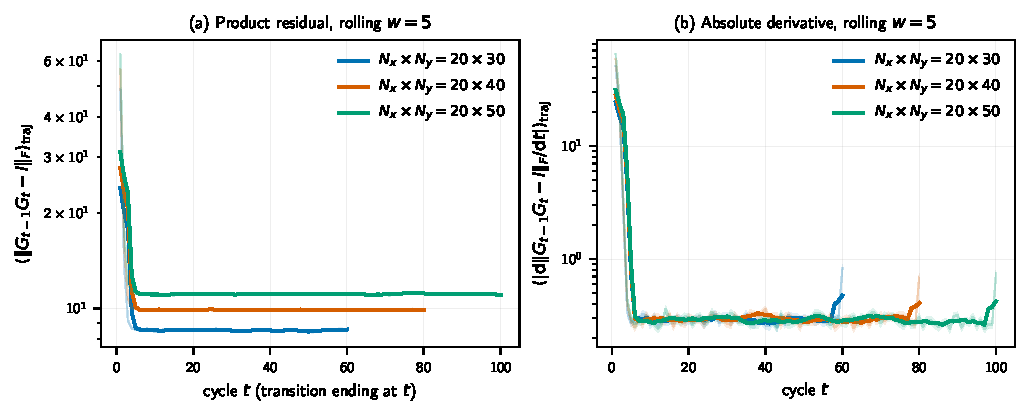
\includegraphics[width=0.98\textwidth]{adjacent_cycle_covariance_product_residual_and_derivative.pdf}
\caption{Pure-state default-initialized streaming ensemble.  Left:
$\overline{\lVert\Qcov_{t-1}\Qcov_t-\mathbf{1}\rVert_F}$, exactly equal to
$\overline{\lVert\Qcov_t-\Qcov_{t-1}\rVert_F}$ by
Eq.~\eqref{eq:productidentity}.  Right: the trajectory mean absolute cycle
derivative.  Thick curves use a centered rolling mean with $W=5$; faint curves
and bands are unsmoothed.  Both axes are logarithmic.}
\label{fig:adjacent}
\end{widefigure}

After the initial drop, the adjacent-cycle residual reaches a size-extensive
plateau: its late means are $8.52$, $9.89$, and $11.09$.  Dividing by
$\sqrt\Vsp$ gives $0.24597$, $0.24730$, and $0.24787$.  This near collapse
shows $O(1)$ RMS covariance motion per cycle even at late times.  Its derivative
becomes small because the \emph{magnitude} of the motion stabilizes; the state
itself does not stop changing.

This observation is fully compatible with convergence to a steady ensemble.
A Markov chain at stationarity keeps moving between states while preserving its
probability distribution.  Therefore
$\lVert\Qcov_t-\Qcov_{t-1}\rVert_F\to0$ is neither required nor expected.
Convergence should instead be tested by stationarity of selected distributions
and by their temporal autocorrelation.

\section{Burn-in, stationarity, and effective ensemble size}
\label{sec:stationarity}

\subsection{Cycle-resolved post-burn-in behavior}

\begin{widefigure}
\centering
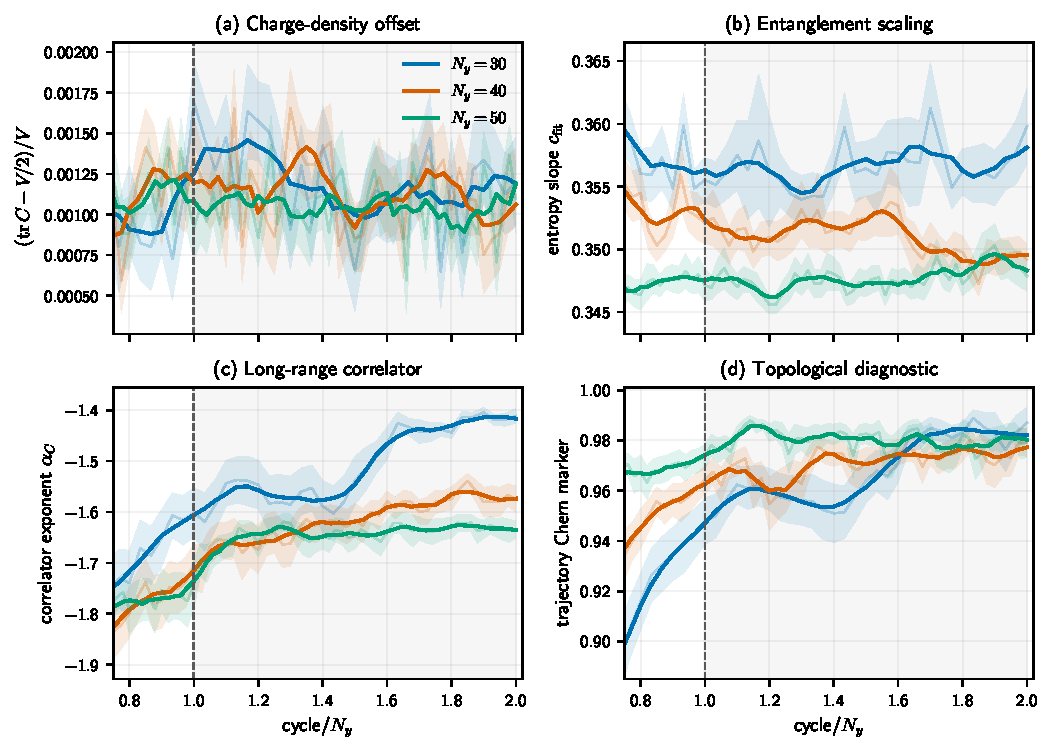
\includegraphics[width=0.84\textwidth]{post_burnin_stationarity_time_series.pdf}
\caption{Default pure-state ensemble near and after the proposed burn-in.
Cycle number is scaled by $N_y$; the dashed line marks $t=N_y$ and the shaded
region is the intended measurement window.  Faint curves and bands show raw
trajectory means and standard errors; thick curves are centered rolling means
with $W=5$ for display only.  The formal block tests use unsmoothed data.
The charge density and entanglement slope are stable, while the smallest sizes
retain visible long-range-correlator and Chern-marker drift.}
\label{fig:stationaritytimeseries}
\end{widefigure}

The four panels in Fig.~\ref{fig:stationaritytimeseries} already show why no
single scalar certifies the entire covariance distribution.  The charge
density is stable to the $10^{-4}$--$10^{-3}$ scale and the entropy slope is
visually flat.  The correlator exponent continues to relax upward, most clearly
for $N_y=30$, and the Chern marker still rises slightly in the same system.

The paired block test makes this quantitative.  Table~\ref{tab:stationarity}
reports raw first-to-second-half differences and the integrated autocorrelation
time.  The $N_y=30$ charge-density interval narrowly excludes zero; its effect
is small, a shift of $2.11\times10^{-4}$ of total capacity.  Entropy-slope
intervals include zero for every size.  Correlator-exponent intervals exclude
zero for $N_y=30,40$ but include zero for $N_y=50$.  The Chern-marker change is
detected only for $N_y=30$.  The normalized covariance-step magnitude is
stationary for all three sizes.

\begin{widetable}
\caption{Post-burn-in stationarity and correlation in the default pure-state
ensemble.  Differences are second-half minus first-half means within
$[N_y,2N_y]$; brackets are trajectory-bootstrap 95\% intervals.  The last two
columns give integrated autocorrelation times in cycles.}
\label{tab:stationarity}
\begin{ruledtabular}
\begin{tabular}{c c c c c c}
$N_y$ & $\Delta c_{\mathrm{fit}}$ & $\Delta\alpha_C$
& $\Delta C_{\mathrm{RS}}$ & $\Tint[c_{\mathrm{fit}}]$
& $\Tint[\alpha_C]$ \\
\hline
30 & $+0.00114\,[-0.00250,0.00502]$
& $+0.1289\,[0.0672,0.1984]$
& $+0.02327\,[0.01106,0.03696]$ & $5.04$ & $14.81$ \\
40 & $-0.00118\,[-0.00342,0.00105]$
& $+0.0689\,[0.0127,0.1293]$
& $+0.00713\,[-0.00256,0.01717]$ & $5.60$ & $20.25$ \\
50 & $+0.000915\,[-0.000329,0.002322]$
& $+0.0207\,[-0.0089,0.0498]$
& $-0.00162\,[-0.00793,0.00450]$ & $6.60$ & $24.10$ \\
\end{tabular}
\end{ruledtabular}
\end{widetable}

\subsection{Stationary does not mean independent}

\begin{widefigure}
\centering
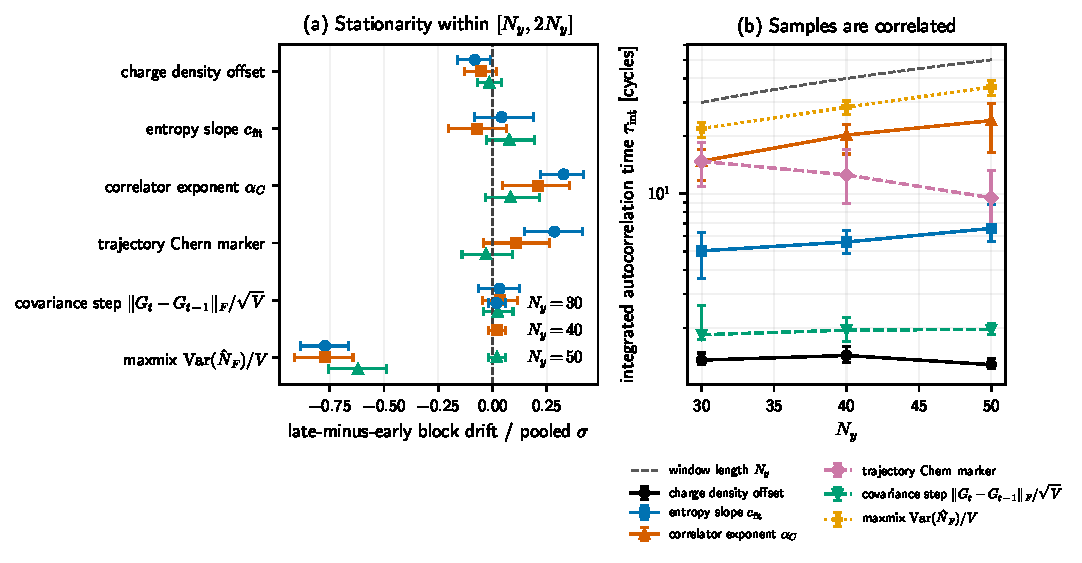
\includegraphics[width=0.94\textwidth]{post_burnin_block_stationarity_and_autocorrelation.pdf}
\caption{Quantitative ensemble test.  Left: second-minus-first-half block drift
divided by the pooled within-window standard deviation; horizontal bars are
trajectory-bootstrap 95\% intervals.  The maxmix quantum charge variance is
included to show that purification remains nonstationary.  Right: integrated
autocorrelation times from trajectory residuals after removing the ensemble
mean separately at each cycle.  The dashed line is the $N_y$-cycle measurement
window length.}
\label{fig:blockacf}
\end{widefigure}

The autocorrelation hierarchy in Fig.~\ref{fig:blockacf}(b) is physically
informative.  The pure-state total-charge density has
$\Tint=1.35,1.43,1.28$ cycles; the covariance-step magnitude has
$1.84,1.94,1.96$ cycles.  The entanglement slope is correlated over
$5.04,5.60,6.60$ cycles.  The long-range correlator exponent is much slower:
\begin{equation}
 \Tint[\alpha_C]=(14.81,20.25,24.10)
 \simeq(0.494,0.506,0.482)N_y.
 \label{eq:correlatortauscaling}
\end{equation}
The three points are consistent with a roughly linear dependence over the
available range, although they are not enough for a controlled dynamical
exponent.  This slow temporal mixing is the ensemble counterpart of the
algebraic wall purification.

Over the inclusive windows of $31,41,51$ cycles, the effective counts per
trajectory are therefore about $6.16,7.32,7.73$ for the entropy slope but only
$2.09,2.02,2.12$ for the correlator exponent.  Multiplying by 100 independent
trajectories gives roughly $616,732,773$ and $209,202,212$
independent-equivalent samples, respectively.  Every retained cycle improves
an estimator, but adding one cycle does not add one independent wall sample.

For the maxmix quantum charge variance,
$\Tint=21.9,28.3,36.1$ cycles and the standardized early-to-late drift is large.
This is precisely the behavior of an ongoing purification transient.  Its
cycles should not be pooled as a steady ensemble even though the same cycle
range is convenient for displaying purification.

\subsection{What can be claimed about the ensemble}

The evidence supports the following statement:
\begin{quote}
After a burn-in, cycle-resolved states are retained as samples of a temporally
correlated Born-rule ensemble.  Stationarity is checked by comparing early and
late blocks of the measurement window, and statistical uncertainties are
computed by resampling trajectories or otherwise accounting for integrated
autocorrelation.  Entanglement observables are stationary after an $N_y$ burn-in
for the tested sizes, while the smallest systems retain measurable drift in
long-wavelength wall correlations.
\end{quote}
This claim is empirical and observable-resolved.  It does not establish equality
of the full probability distribution over all covariance matrices, which would
require a much more demanding two-sample test in a high-dimensional state
space.

\section{A systematic convergence protocol}
\label{sec:protocol}

A good convergence timescale should be defined by the observable and the
target precision, not selected from a visually flat curve.  The following
procedure is supported by the present data.

\begin{enumerate}
  \item Choose observables that cover the sectors relevant to the final claim:
  a global scalar, an active-bulk diagnostic, a wall-localized diagnostic, and
  any topological or long-range correlation statistic that will appear in the
  paper.
  \item For each observable $O$, choose a physically interpretable tolerance
  $\epsilon_O$.  Define $T_O$ by a sustained threshold or, for a quantity with a
  nonzero plateau, by a sustained rate threshold.
  \item Set the provisional burn-in to
  \begin{equation}
   T_{\mathrm{burn}}=\max_O T_O.
   \label{eq:burninmax}
  \end{equation}
  For an algebraic wall mode, document the tolerance explicitly because
  Eq.~\eqref{eq:tolerancewalltime} makes $T_O$ tolerance dependent.
  \item On the proposed measurement window, compare its first and second
  halves using paired trajectory block means.  Increase the burn-in if a
  practically important observable exhibits statistically resolved drift.
  \item Estimate $\Tint[O]$ and report either trajectory-block bootstrap
  errors or $N_{\mathrm{eff}}$.  Select the measurement-window length from the
  slowest relevant $\Tint$, not from the number of saved cycles alone.
  \item Repeat at multiple $N_y$ while holding the other geometry fixed before
  claiming a scaling law for $T_{\mathrm{burn}}$ or $\Tint$.
\end{enumerate}

Applied here, this protocol distinguishes three uses of $N_y$:
\begin{itemize}
  \item As a \emph{burn-in}, $N_y$ is conservative for $N_y=50$ and for
  global/entanglement observables.  For $N_y=30,40$, it begins before the
  slowest wall sector is fully stationary according to the correlator exponent.
  A conservative finite-size rule for the present dataset is
  $T_{\mathrm{burn}}\gtrsim\max(N_y,50\text{--}60)$ when long-wavelength wall
  observables matter.
  \item As a \emph{measurement-window length}, $N_y$ is well motivated because
  the slow correlator has $\Tint\approx0.49N_y$, yielding about two
  independent-equivalent wall samples per trajectory.  A shorter $O(1)$ window
  would lose effective wall statistics as $N_y$ grows.
  \item As an \emph{endpoint}, $2N_y$ is sufficient for the observed
  $0.01$-bit wall-entropy criterion and clearly sufficient for the global
  Frobenius criterion.  It is not an assertion of arbitrary-precision
  convergence.
\end{itemize}

This also answers whether cycle time must scale with $N_y$.  The global
purification burn-in need not scale with $N_y$ over the tested range.  The
wall's temporal autocorrelation, however, is approximately proportional to
$N_y$, so the amount of simulation required for a fixed number of
independent-equivalent wall samples does scale with $N_y$.  Burn-in and sampling
cost are different questions.

\section{Interpretation and limitations}
\label{sec:limitations}

The combined evidence supports a physical picture of fast bulk contraction and
a slowly purifying critical wall.  Global norms rapidly approach their pure
ceiling because the bulk dominates the volume.  Boundary-resolved entropy and
reduced-covariance motion retain algebraic tails.  Once the marginal
distribution has settled, the circuit keeps generating distinct trajectory
states; long-wavelength wall information remains correlated across many cycles.

Several limitations constrain the language:
\begin{enumerate}
  \item The $N_x=20$ global campaign has only three circumferences.  Constancy
  of $\Tconv^{(F)}$ over $N_y=30$--$50$ is not an asymptotic theorem.
  \item The spatial covariance pilot has ten trajectories and four snapshots.
  Its $R_x$ ratios are strong descriptive evidence, not a fitted dynamical
  exponent.
  \item The wall-entropy geometries do not form a clean one-parameter size
  series.  They establish wall/bulk separation and power-law time dependence,
  but not a system-size scaling exponent for the wall threshold time.
  \item Hard domain-wall truncation enforces much of the near-zero exterior.
  Claims should concern localization within the active slab unless compared
  against an untruncated control.
  \item Stationarity tests cover selected observables, not the full covariance
  distribution.  Failure to detect drift is not proof of exact stationarity.
  \item The centered rolling average with $W=5$ is a visualization aid.  It is
  not additional data, and formal block comparisons use raw cycle values.
\end{enumerate}

The most important semantic limitation is the distinction between nonlinear
trajectory observables and observables of the averaged correlation matrix.
For example, $\overline{C_G}$, the Born average of trajectory-resolved Chern
numbers, is generally not $C_{\overline G}$, the Chern number computed after
averaging $G$.  The present Chern stationarity test uses the former.

\section{Reproduction checklist}
\label{sec:reproduction}

The authoritative analysis root is
\path{analysis_outputs/total_charge_variance_cycle_derivative/}
within the \path{colab_charge_fluctuations} package.  Its manifest records
the complete source-file list, estimator definitions, campaign identifiers,
and output paths.  The original analysis notebook is
\path{plot_total_charge_variance_and_derivative_cpu.ipynb}.

The two stationarity figures and their tables are regenerated locally by
\path{make_ensemble_sampling_figures.py}.  The script reads the archived
streaming fits, scalar metrics, local charge arrays, and maximally mixed total
charge variance; it does not rerun dynamics.  It checks a complete
$100\times2N_y$ grid for every observable and size, uses 2000 trajectory
bootstrap repetitions with seed 314159, and writes:
\begin{itemize}
  \item \path{post_burnin_stationarity_time_series.csv},
  \item \path{post_burnin_stationarity_autocorrelation_summary.csv},
  \item the corresponding PDF and PNG figure pairs, and
  \item \path{analysis_manifest.json} beside this note.
\end{itemize}
All other figures are the archived PDFs emitted by the characterization
notebook.  Compilation uses RevTeX~4.2 in two-column PRB format.

\section{Conclusions}

The charge and covariance data admit a coherent but nontrivial convergence
story.  Global purification is fast and essentially independent of $N_y$ over
the explored range.  The active bulk contracts exponentially on an $O(1)$
cycle scale.  The domain wall purifies algebraically and controls the longest
transient and autocorrelation scales.  Ensemble-mean occupancy bias and
trajectory-to-trajectory occupancy fluctuations are sharply wall localized,
while within-trajectory quantum charge variance is spread throughout the
active slab.

The production convention of burning in for $N_y$ cycles and measuring on
$[N_y,2N_y]$ is therefore sensible, but its meaning should be stated precisely.
At cycle $2N_y$, the observed wall entropy is below $0.01$ bits per cell and
global covariance purification is long complete.  During the measurement
window, each cycle can be retained as a Born-rule ensemble sample once the
observable's marginal distribution passes a stationarity check.  The cycles
are not independent: the slow correlator contributes only about two
independent-equivalent samples per trajectory over an $N_y$-cycle window.
This distinction permits use of all saved cycles without overstating the
statistical sample size.

\begin{thebibliography}{5}
\bibitem{Bhuiyan2026}
A.~Bhuiyan, H.~Pan, and C.-M.~Jian,
Free-fermion dynamics with measurements: Topological classification and
adaptive preparation of topological states,
Phys. Rev. Research \textbf{8}, 023147 (2026).

\bibitem{Calabrese2004}
P.~Calabrese and J.~Cardy,
Entanglement entropy and quantum field theory,
J. Stat. Mech. P06002 (2004).

\bibitem{Sokal1997}
A.~D.~Sokal,
Monte Carlo methods in statistical mechanics: Foundations and new algorithms,
in \emph{Functional Integration: Basics and Applications} (Plenum, New York,
1997).
\end{thebibliography}

\end{document}
